\hthree{Die "App"-Klasse}\label{sec:app}

Die "App"-Klasse übernimmt die Verwaltung aller Endpunkte.  

\begin{figure}[H]
    \centering
    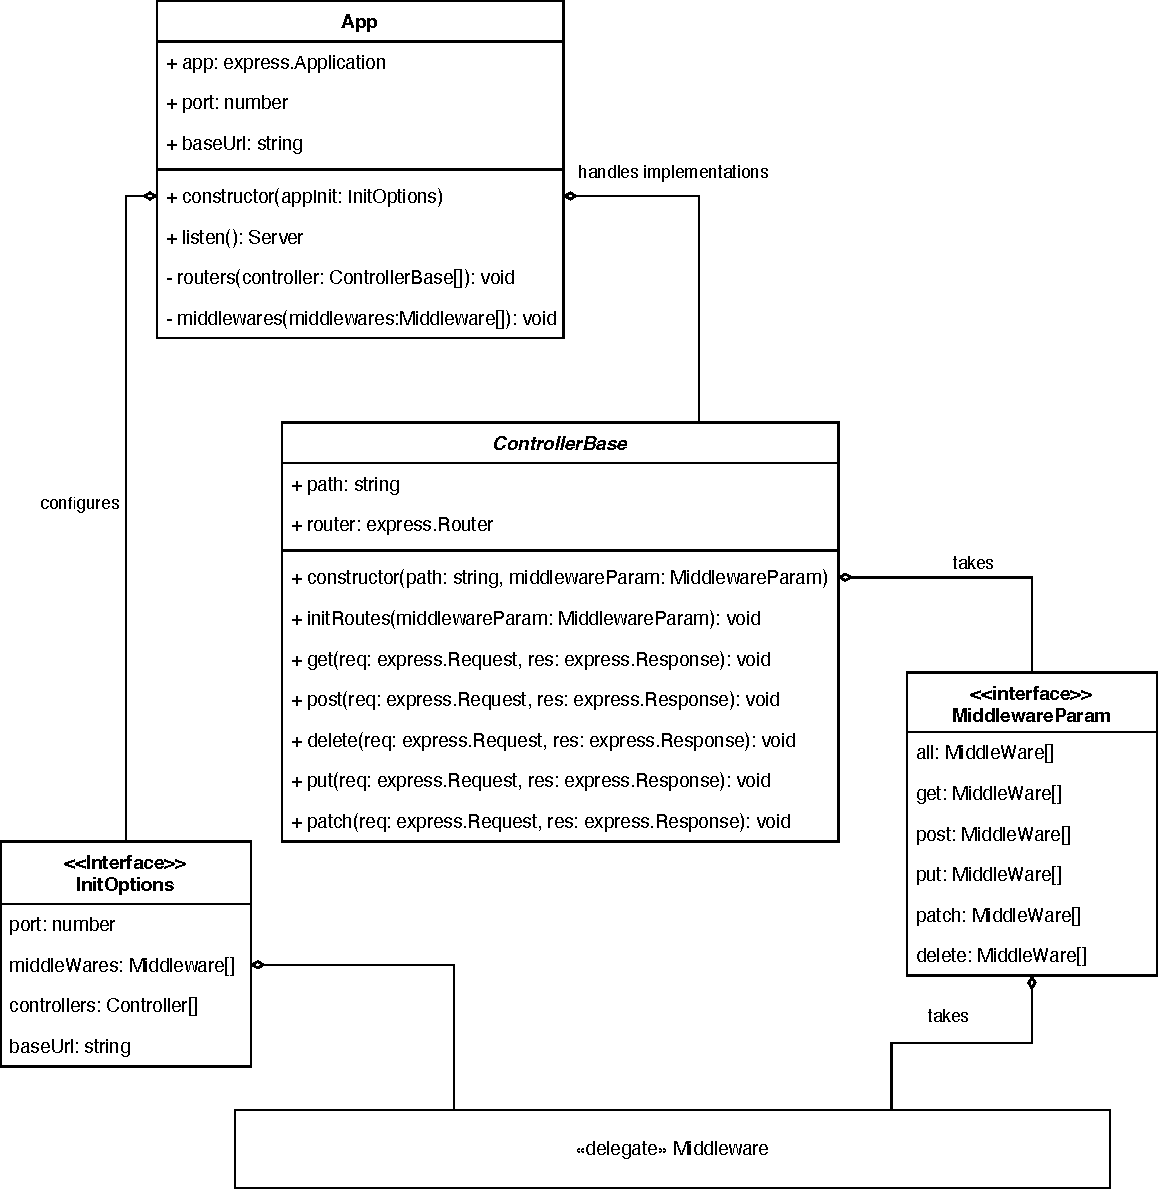
\includegraphics[width=\textwidth]{media/APITemplate/apiArchitecture.svg.pdf}
    \caption{UML Diagramm der API-Architektur}
    \label{fig:apiUML}
\end{figure}

\pagebreak

Im Konstruktor der App-Klasse können verschiedene Optionen mitgegeben werden:

\hfive{"Port"}

Durch die Port-Option kann angegeben werden, auf welchem Port die API HTTP-Requests annehmen soll. Standardmäßig ist dies auf die Umgebungsvariable "PORT" gesetzt. Falls diese nicht gesetzt ist, wird der Port 3001 verwendet.

\hfive{"Controllers"}

Die "Controller" werden als Array von "Controller"-Objekten übergeben und repräsentieren einen Endpoint (siehe Kapitel "Controllers" \ref{sec:controller}).

\hfive{"Middlewares"}

Dies ist ein Array an "Middlewares", welche bei jedem Request vor den "Controllern" ausgeführt werden (siehe Kapitel "Middleware" \ref{sec:middleware}).

\hfive{"Base-URL"}

Durch diesen String kann der Root-Pfad definiert werden. Standardmäßig ist dieser auf "{\ttfamily /}" gesetzt. Bei ZELIA ist dieser auf "{\ttfamily /api}" konfiguriert worden, da alle API bezogenen Anfragen auf den Pfad "{\ttfamily /api}" gehen.

Um eine Instanz der App-Klasse zu erstellen, muss diese importiert werden. Danach kann die "App" mit ihren registrierten "Controllern" und "Middlewares" instanziiert werden. Damit die "App" auf dem angegebenen Port gestartet wird, muss die "listen"-Methode aufgerufen werden.

\typescript{code/APITemplate/appusage.ts}{Verwendung der App-Klasse}